\documentclass[a4paper, 12pt,oneside]{article} 
%\documentclass[a4paper, 12pt,oneside,draft]{article} 
\usepackage{preamble}
\usepackage{pythonhighlight}

%--------------------- ACTUAL FILE ---------------------- %
\begin{document} 
%%%
	%\setcounter{page}{1}
	\begin{center}
	    \Large
	    \textbf{HMC : When is it worth over RWMC ?} 
	    \vspace{0.4cm}
	    \large

		Course : Stochastic Simulation \\
	    Students : Aude Maier \& Tara Fjellman \\
	    \small{Fall 2024}
	\end{center}

	\section{Introduction}
	\section{Core Theory}
		\subsection{RWMC}
		A common shortfall of the simple random walk Metropolis proposal in the Metropolis-Hastings algorithm is the slow exploration rate of the state space. Much effort has been devoted in recent years to devise proposals with more efficient exploration rates (i.e "distant" proposals).
		\subsection{HMC}
			\subsubsection{The Algorithm}
			HMC considers the Hamiltonian dynamics associated to a Hamiltonian function $H$ : $\mathbb{R}^d \times \mathbb{R}^d \rightarrow \mathbb{R}, H=H(q, p)$, where the position variables $\{q_i\}$ are the random variables we want to sample and ``fictitious'' momentum variables $\{p_i\}$ are introduced. 
			
			The Hamiltonian dynamics are dictated by the equations
			\begin{gather}
			\frac{d q_i}{d t} =\frac{\partial H}{\partial p_i}, \\
			\frac{d p_i}{d t} =-\frac{\partial H}{\partial q_i},
			\end{gather}
			for $i=1, \ldots, d$. In general, the above equation can be understood as a conservation of the total energy of a system in time.
			
			Samples of the $q$ vector are then obtained by constructing a Markov Chain Monte Carlo algorithm with given invariant density $\pi(q)$ on the position variables $\left(q_1, \ldots, q_d\right)$. To do so, we introduce the potential energy $U(q)=-\log \pi(q)$, a kinetic energy $K(p)=\sum_{i=1}^d \frac{p_i^2}{2 m_i}$, for some mass parameters $m_i, i=1, \ldots, d$, and the Hamiltonian $H(q, p)=U(q)+K(p)$. Having introduced these functions, we can then simulate a Markov chain in which each iteration re-samples the momentum, evolves the Hamiltonian system for a certain time, and then performs a Metropolis-type acceptance-rejection step on the new position vector. More concretely, we consider the so-called Gibbs measure, given by
			$$
			G(q, p)=\frac{1}{Z} e^{-H(p, q)},
			$$
			where $Z$ is the (unknown) normalizing constant. Notice that such a Gibbs measure naturally factorizes as:
			$$
			G(q, p)=\frac{1}{\tilde{Z}} e{-U(q)} \frac{1}{\prod_{i=1}^d \sqrt{2 \pi m_i}} e{-K(p)}
			$$
			
			where $\frac{1}{Z} e^{-U(q)}$ is the probability density we are interested in sampling from, whereas the other factor is a multivariate Gaussian distribution $N(0, M)$ with $M=\operatorname{diag}\left(m_1, \ldots, m_d\right)$. Given the state $q^n$ at iteration $n$, the idea of the algorithm is then to sample a momentum vector $p^n$ from $N(0, M)$, and compute $H\left(q^n, p^n\right)$. The Hamiltonian system is then evolved starting from $q(0)=q^n, p(0)=p^n$, on a time interval $[0,T]$ using the dynamical equations for some arbitrary final time $T$, to obtain $(q(T), p(T))$. This state is then taken as the proposal state in a Metropolis-Hastings step to generate the new state $q^{n+1}$. For many problems of modern relevance, it is not possible to compute the dynamics exactly and numerical discretization is needed. A convenient time discretization scheme is the Verlet's method: the time interval $[0, T]$ is divided into $N_t$ intervals of size $\epsilon>0$ and for each particle $i$ the position $q_i$ and momemtum $p_i$ are updated as follows			
			\begin{align}
			& p_i(t+\epsilon / 2)=p_i(t)-(\epsilon / 2) \frac{\partial U(q(t))}{\partial q_i}, \\
			& q_i(t+\epsilon)=q_i(t)+\epsilon \frac{p_i(t+\epsilon / 2)}{m_i}, \\
			& p_i(t+\epsilon)=p_i(t+\epsilon / 2)-(\epsilon / 2) \frac{\partial U(q(t+\epsilon))}{\partial q_i}.
			\end{align}	
			%The main steps of the Hamiltonian Monte Carlo algorithm using Verlet's method are outlined in Algorithm 1. There, $N$ is the length of the chain, $\epsilon$ the time step in Verlet's method, and $T$ the final integration time.
			\subsubsection{Acceptance Rate}
			To explore how the acceptance rate behaves in HMC, we must consider the quantity \newline $\exp \left[U\left(q^n\right)+K\left(p^n\right)-U\left(q^*\right)-K\left(p^*\right)\right]$ which appears in the expression for $\alpha$ in the Metropolis-Hastings acceptance probability. Using the definition $H(q, p)=U(q)+K(p)$ we can write this quantity as:
			\begin{gather}
				\exp \left(U\left(q^n\right)+K\left(p^n\right)-U\left(q^*\right)-K\left(p^*\right)\right) = \exp \left[H\left(q^n, p^n\right)-H\left(q^* p^*\right)\right].
				\label{eq:HMC-acceptance-rate} 
			\end{gather}
			Since the Hamiltonian is conserved under the Hamiltonian dynamics :
			\begin{align}
			\frac{d H}{d t}=&\sum_i \frac{\partial H}{\partial p_i} \frac{d p_i}{d t}+\sum \frac{\partial H}{\partial q_i} \frac{\partial q_i}{d t} \\
			=&-\sum_i \frac{\partial H}{\partial p_i} \frac{\partial H}{\partial q_i}+\sum_i \frac{\partial H}{\partial q_i} \frac{\partial H_i}{\partial p_i} = 0,
			\end{align}
			we find by using this in \ref{eq:HMC-acceptance-rate} that if integration is exact, the acceptance rate is always 1.

			Under the assumption that the Hamiltonian dynamics is discretised, conservation is there in the best case on average. This implies the acceptance rate will be less than 1. 
			\subsubsection{Convergence to Target Distribution}
			\paragraph{Gibbs measure invariance}
			Under the assumption that there is no numerical error, we want to prove that the Gibbs measure is invariant for the chain generated by the hamiltonian dynamics.
	
			This is equivalent to saying that the Gibbs measure $\pi$ is the same before and after an evolution of $t$ seconds from the hamiltonian dynamics. 
			To prove this we first introduce hamiltonian dynamics operators $\phi,\Phi$ acting respectively on the phase space and the Gibbs measure : $\phi_t(q_s,p_s)=(q_{s+t},p_{s+t});\Phi_t[\pi_s]=\pi_{t+s}\quad \forall t\in\mathbb{R}$.
			The statement we want to prove can then be expressed as 
			\begin{gather}
				\Phi_t[\pi_s](D)=\pi_{s+t}(D)\quad \forall D\in\mathcal{B}(\Omega),\forall s,t\in\mathbb{R},
				%P(T_t(q,p)\in D_s)=
				%P((q,p)\in T_{-t}(D_s))=
				%P((q,p)\in D_s)=\pi(D_s),
				%P((q,p))=\int_{\Omega} K((q,p),D_s) G(q,p) \ dq dp=\pi(T_t[D_s]),
			\end{gather}
			with $\Omega$ the phase space.
	
			We can now write the left hand side of the equation as
			\begin{align}
				\Phi_t[\pi_s](D)&=\int_D \pi_{s+t}(q,p)\ dqdp \\
					&=\int_{\phi_{-t}(D)}\pi_{s}(q,p)\ dqdp \\
					&=\pi_s(\phi_{-t}(D)).
			\end{align}
			The final result is obtained using the fact that volumes in phase space are preserved by the hamiltonian dynamics (in conservative systems). This result is known as Liouville's theorem, but is mentioned as theorems 2.3 in [cite].
			%K:\Omega \times D\to [0,1]$ the transition kernel of the chain, $G(q,p)$ the Gibbs measure, and $T_t[\cdot]$ the hamiltonian time evolution operator defined by $T[(q_s,p_s)]=(q_{s+t},p_{s+t})$.
	
			This implies specifically that $q_k\sim\pi$ for all $k\in\mathbb{N}$ if $q_0\sim \pi$. 
	
			If the dynamics is discretised with the Velocity Verlet algorithm, the volume in phase space is preserved up to a small error, which is why the algorithm is used in practice [cite wikipedia].
	\section{Exploring a 2D example}
		\subsection{Context}
		In this section we explore the performance of the presented algorithms on a 2D example. The target distribution is taken as $f_1(q_1,q_2)=e^{-\alpha(q_1^2+q_2^2-0.25)^2}$, with $\alpha>0$ a parameter. This unormalised density is represented in figure \ref{fig:alpha-density} for two different values of $\alpha$.
        \begin{figure}[htb]
            \centering
                \vspace{0em}
                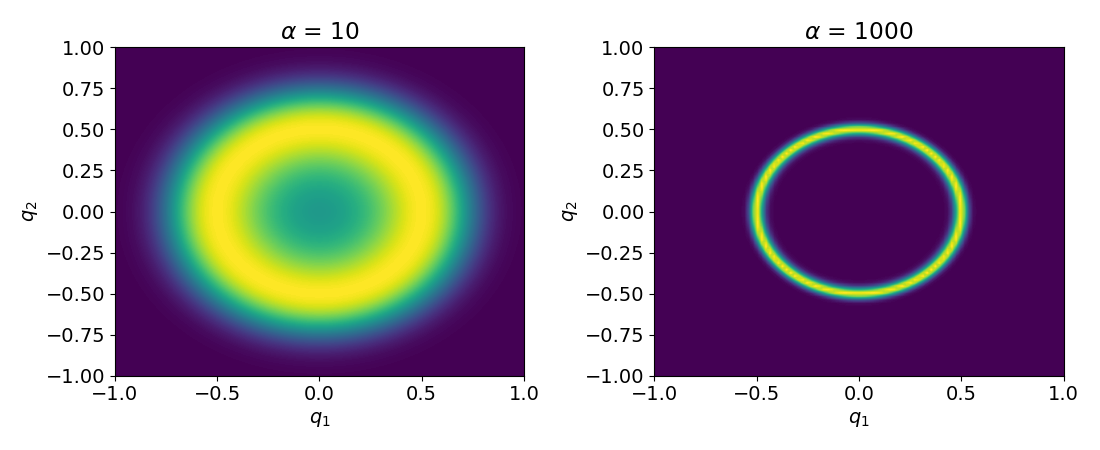
\includegraphics[width=0.9\textwidth]{alpha_density}
                \caption{Density considered in this section for two different values of $\alpha$.}
                \label{fig:alpha-density}
        \end{figure}
		As it can be seen, the density has the shape of a doughnot and $\alpha$ controls its thickness. We expect the $\alpha=1000$ case to be more difficult to sample from than the $\alpha=10$ case, as the density is more localised.
		\subsection{RWMC Solution}
			As seen previously, the RWMC algorithms only depends on the step size. We can therefore easily find the best RWMC sampler version by exploring the impact of the step size on performance. 
			
			Here and in the following, we decide to quantify performance throught the computation of a similarity based on the Jensen-Shannon divergence. This choice allows us to feed in a discretised version of $f_1$ (which we can normalise) and the empirical distribution of the samples generated by the algorithm, and get a similarity measure between the two.

			The similarities associated to 3000 samples for the different step sizes are presented in figure \ref{fig:rwmc-scan}.
			\begin{figure}[htb]
				\centering
					\vspace{0em}
					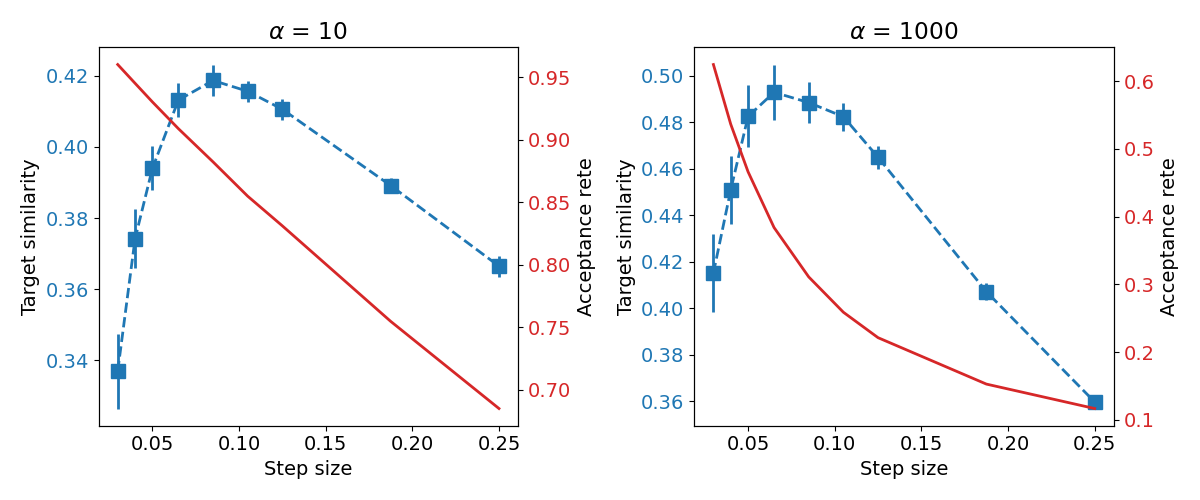
\includegraphics[width=0.95\textwidth]{rwmc_scan}
					\caption{Similarity as a function of RWMC step size for considered values of $\alpha$.}
					\label{fig:rwmc-scan}
			\end{figure}
			Lookng at the plots, it is clear they display a local maxima around 8.5$\times 10^{-2}$ and 6.5$\times 10^{-2}$ for $\alpha=10$ and $\alpha=1000$ respectively. Such a feature is expected as the step size is a tuning parameter that should be chosen to match the scale of the target distribution.
			More precisely, the peak is sharper on its right for the $\alpha=1000$ case, which is consistent with the fact that the density is more localised. 
			The value of the similarity is in all cases $<0.5$, which means that 3000 samples are too few to accurately estimate the target distribution. The value is higher in the $\alpha=1000$ case, which can at first look surprising. Indeed, this case is meant to be harder than the $\alpha=10$ ono. However, since the density is more localised for $\alpha=1000$, there are fewer places where the estimate and the target can differ, which leads to a better similarity. It is therefore important to consider the relative values of the similarities for the different step sizes, rather than the absolute ones.
			Looking at the evolution of the acceptance rate, we see that it is of course monotonically deacreasing with step size. This means that the obtimal value corresponds with the best exploration-acceptance rate trade-off. The acceptance rate is higher and decreases slower for the $\alpha=10$ case, which is consistent with the fact that the density is more spread out. The acceptance rate of the $\alpha=1000$ case associated to the best step size is still around 0.4, which suggests that even this case is still quite easy to sample from (i.e. random proposals are good enough). 
		\subsection{HMC Solution}
			\begin{wrapfigure}[18]{r}{0.6\textwidth}
				\centering
					\vspace{-2em}
					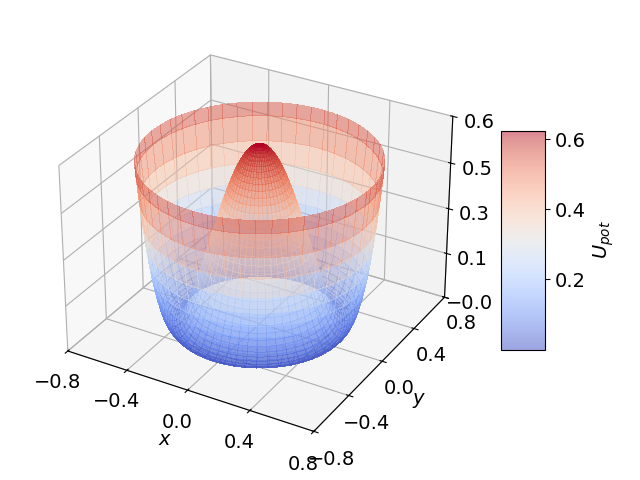
\includegraphics[width=0.57\textwidth]{U_pot_alpha=10}
					\caption{Potential energy landscape associated to HMC algorithm for $\alpha=10$. Version for $\alpha=1000$ is identical, except scales are scaled by a factor of 100.}
					\label{fig:U-pot-alpha=10}
			\end{wrapfigure}
			Before exploring the impact of the different parameters of the HMC algorithm, we first present the potential energy landscape associated to the algorithm for this specific problem. The landscape is presented in figure \ref{fig:U-pot-alpha=10}. 
			The landscape has polar symmetry, meaning the trajectories will be some sort of isotropic oscillations. It has global minima at a radius of $\sqrt{0.25}=0.5$ away from the centre and a local maxima at the origin. The only difference in the landscape for $\alpha=1000$ w.r.t. the $\alpha=10$ one is the scale of the potential. This means that the $\alpha=1000$ will give rise to stronger potential forces, which translates the fact that the density is more localised. 
			\subsection{Impact of Mass Scale}
			The first parameter we explore is that of the mass. We split this in terms of the mass scale and the mass symmetry. We do not consider the impact of off-diagonal terms as this would make the report too long and was not suggested in the statement. 

			What we expect to see is that the mass scale will control the speed of the dynamics (by affecting the particle's inertia).
			The similarities associated to 3000 samples for the different mass scales are presented in \ref{fig:mass-scan}.
			\begin{figure}[htb]
				\centering
					\vspace{0em}
					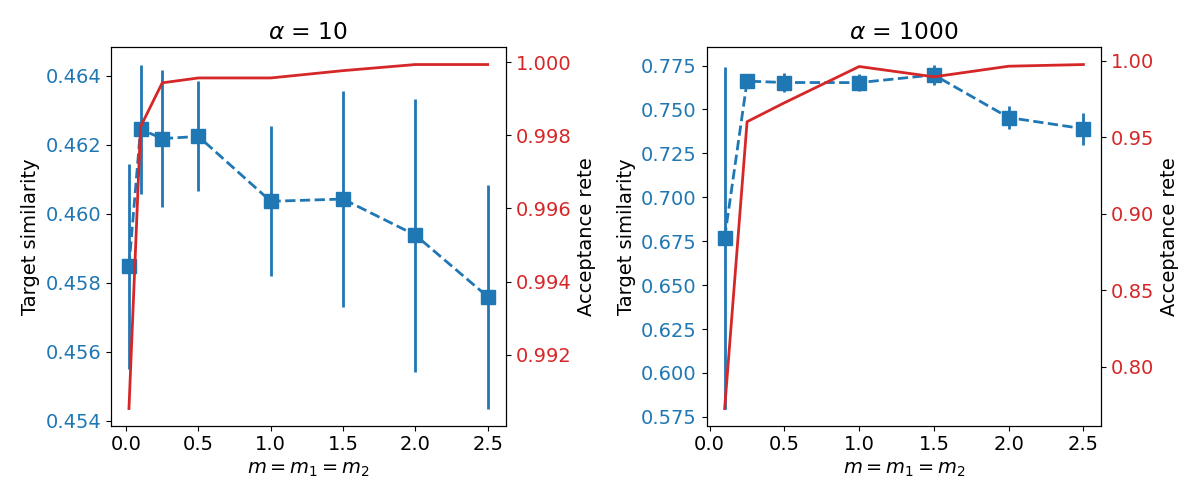
\includegraphics[width=0.95\textwidth]{mass_scan}
					\caption{Similarity as a function of HMC mass scale for considered values of $\alpha$.}
					\label{fig:mass-scan}
			\end{figure}
			In this case, both plots look qualitatively similar : the similarity admits a global maxima at some value of the mass scale, and worsen on both sides of it. The acceptance rate on the other hand stays really close to $1$, probably due to the $\Delta t$ being quite generosly choosen. The decrease in performance is therefore due to the fact that the particle explores less well the space. We can easily make sense of it for higher values of the mass, as the particle will be more inert and therefore less likely to explore the space. For lower values of the mass, the particle will be more reactive to forces, so the decrease in exploration can seem counter-intuitive. We could however immagine that if the mass is too low, the particle will be more likely to oscillate around the minima, and so not explore well other parts of the domain.
			
			There are a couple of difference worth noting between the $\alpha=10$ and $\alpha=1000$ cases. The first is that the second case has its peak around a higher value of the mass. This is consistent with the fact that the forces are stronger, and therefore it requires more inertia to explore well the space (when integration time is fixed). 
			% (ASK AUDE IF MAKES SENSE). 
			The second difference is that the $\alpha=1000$ case seems to suffer more from the mass scale being too large. The reason is probably similar, given in addition that the characteristic time is shorter for this case (and therefore the same absolute change in travelled distance is more important).
			\subsection{Impact of Mass Symmetry}
			What we expect to see is that mass symmetry will control the isotropy/anisotropy of inertia. Indeed, if masses are different, the particle will have different inertia in different directions, which will affect the shape of the trajectories. In some direction the particle will react more quickly to forces, while in the other it will be more inert.
			In our case, the target distribution (and therefore potential landscape) is isotropic. We would therefore expect that better results are obtained with symmetric masses. If the main axis of motion were not to be orthogonal, we would even expect to find an advantage in properly choosing (non-zero) off-diagonal terms too. 

			We tried to gain insight into this with help of \ref{fig:mass-sym}, in which the similarities associated to 3000 samples for both symmetric and asymmetric masses are represented.
			\begin{figure}[htb]
				\centering
					\vspace{0em}
					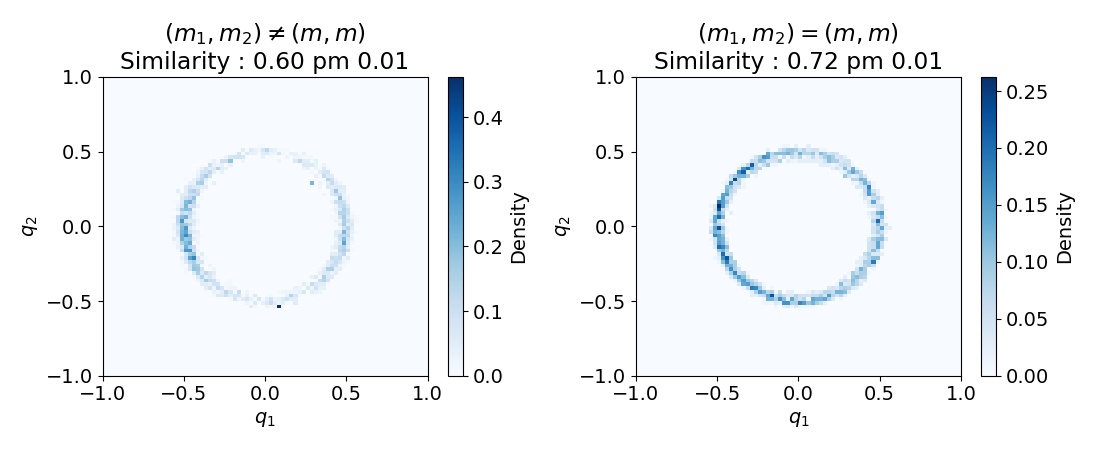
\includegraphics[width=0.95\textwidth]{mass_sym}
					\caption{Similarity for HMC samplers with asymmetric and symmetric masses for $\alpha=1000$.}
					\label{fig:mass-sym}
			\end{figure}
			A first look at the plot shows that the similarity is slightly better for the symmetric mass case. 
			More precisely in our case, the plot associated to anisotropic masses reveils that left and right areas of the distributions are sampled more than the top and bottom ones. This seems to be a consequence of the fact that in that example $m_1>m_2$ (as the particle's inertia is stronger along the horizontal axis). 
			\subsubsection{Impact of Integration Time}
			The next parameter we explore is integration time. For this parameter, we expect the optimal value to be the one that allows the sampler to explore the whole space, without being excessively long (as it would slow down sampling).
			The similarities associated to 3000 samples for the different integration times are presented in figure \ref{fig:t-scan}.
			\begin{figure}[htb]
				\centering
					\vspace{0em}
					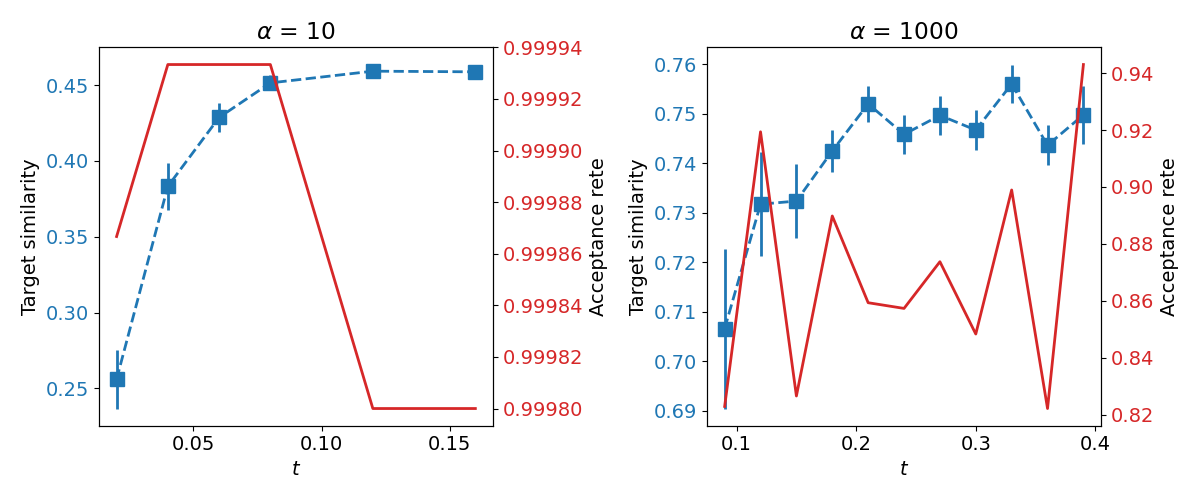
\includegraphics[width=0.95\textwidth]{t_scan}
					\caption{Similarity as a function of HMC integration time for considered values of $\alpha$.}
					\label{fig:t-scan}
			\end{figure}
			From a qualitative point of view, the behaviour is the same for both settings : similarity increases as a function of $t$ untill a plateau around $t=9\times 10^{-2}$ is reached. Looking more closely, it seems that the curve is sligthly more noisy for the $\alpha=1000$ case.
			%Curiously, we observe a steady decrease in acceptance rate for the $\alpha=10$ case and something that looks like a dampt oscillation for the $\alpha=1000$ one. This could be due to the characteristic time of oscillation being of the same order as the time differences considered. 
			\subsection{Impact of $\Delta t$}
			We now turn to analysing the impact of the time step. This parameter is important as it controls the accuracy of the integration. The goal is to find the largest time step that allows for accurate integration, as this will speed up the sampler while allowing it to accept proposals frequently.

			The similarities associated to 3000 samples for the different time steps are presented in figure \ref{fig:dt-scan}.
			\begin{figure}[htb]
				\centering
					\vspace{0em}
					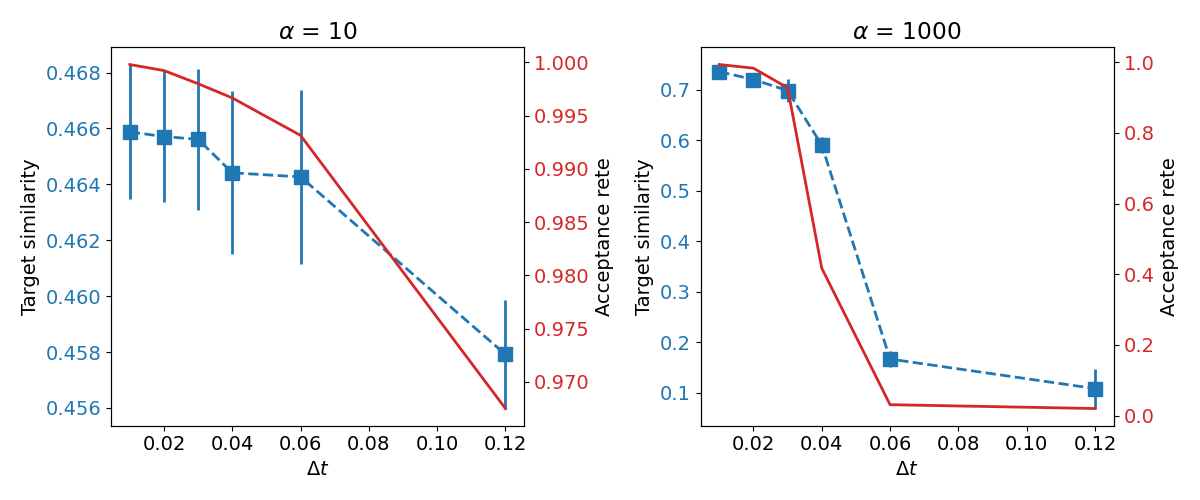
\includegraphics[width=0.95\textwidth]{dt_scan}
					\caption{Similarity as a function of HMC time step for considered values of $\alpha$.}
					\label{fig:dt-scan}
			\end{figure}
			The first characteristic feature the two plots share is the monotonous behaviour of the acceptance rate. Indeed, as mentionned before, by making $\Delta t$ grow, the simulation does not exactly leave the Hamiltonian invariant, and therefore makes the acceptance rate decrease. This in turn can affect the similarity, as fewer samples are obtained and therefore these represent the target distribution less precisely. This happens particularly noticepbly in the $\alpha=1000$ case, where we reach a really low acceptance rate at $\Delta t=6\times 10^{-2}$. This can be interpreted as due to the characteristic time being shorter than in the $\alpha=10$, and therefore requiring finer resolution. Indeed, for $\alpha=10$ good acceptance rate is mantained in term of accpetance rate and target similarity even when a single timestep of size $t$ is taken. This makes sense since the obtained algorithm is still some sort of upgraded version of RWMC where the general direction of the step is choosen smartly and RWMC already performed well over quite a broad domain of step sizes.   
			\subsection{Comment on interractions between parameters}
			In the previous sections, the analysis of HMC's parameters was limited to a one-factor-at-a-time study. This was motivated by the non-exhaustive character of the report and the fact that meaningfull insights were associated to these longitudinal analyses. 
			
			In reality however, each parameter of course does not act in a vacume. More specifically, qualitative explorations of simulations reveiled for example that increasing mass slightly, required longer integration times for space-exploration to occur, and often allowed for a larger $\Delta t$ to be used. The symmetric finding was found for lowering mass slightly. This has practical implications in finding global optimal choice of parameters. Indeed, when grid search for the parameters is untractable (i.e. in high dimensions), these interractions between the parameters make it hard to find globally optimal values. Our intuition is that in these cases one can proceed in the following way to find ``good enough'' parameters ``easily'' : 
			\begin{enumerate}
				\item use assumptions on the potential to choose structure for the mass (isotropy, anysotropy etc.) and possibly do the same to derive a characteristic time for the oscillation,
				\item select the locally optimal mass scale after having set  the time and $\Delta t$ generously : the time larger than optimal (guaranteeing good mixing) and $\Delta t$ smaller than optimal (granting precise integration),
				\item with the new mass matrix, select the locally optimal integration time (shortest one preserving good enough mixing),
				\item finally select the locally optimal $\Delta t$ (the biggest for which the acceptance rate is good enough).
			\end{enumerate}
			We do not expect this approximate tuning of the parameters to be a problem given that alternatives like RWMC breakdown in high dimensions. A locally optimal selection of HMC parameters will probably still lead to a much more efficient sampler.   
		\subsection{RWMC and HMC Comparison}
		\subsubsection{Target-Similarity as a Function of Sample-Size}
		To determine which algorithm is best to use for the studied 2D example, it is interesting to compare the results obtained with optimised versions of the RWMC and HMC algorithms as a function of sample size (matching the number of function evaluations). We do this in \ref{fig:nsamples-evolution}.
		%Note that the optimal HMC parameters for the $\alpha=10$ case were not found following the algorithm described above. Indeed in this special case, the problem is so simple that taking a single timestep of size $t$ is enough to get a good similarity. The improvement obtained by taking more timesteps is therefore irrelevant when compared to the computation burden.
		\begin{figure}[htb]
			\centering
				\vspace{0em}
				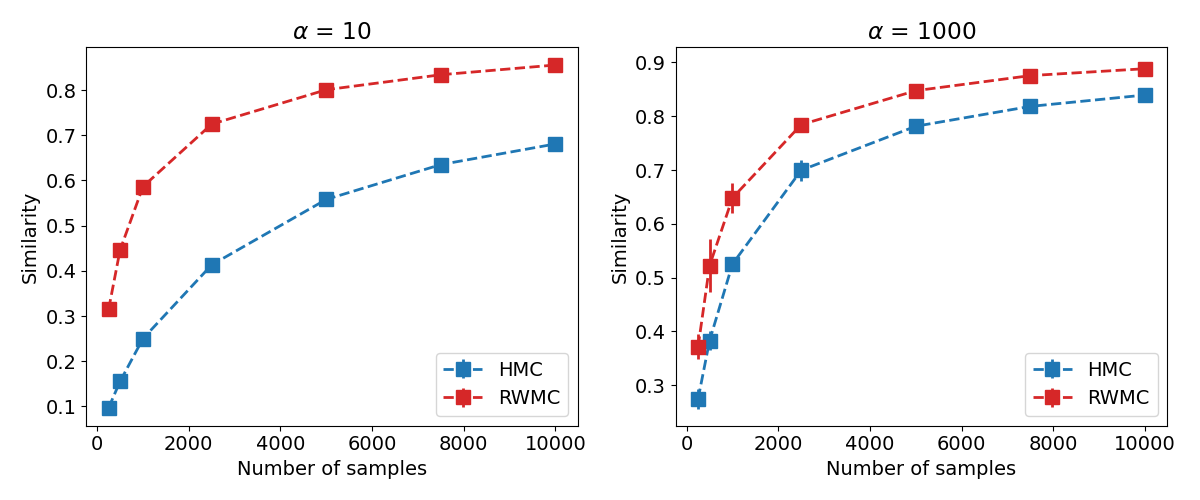
\includegraphics[width=0.9\textwidth]{nsamples_evolution}
				\caption{Similarity as a function of sample-size for RWMC and HMC samplers and considered values of $\alpha$. The sample-size represented on the x axis is that associated to the HMC sampler. The associated RWMC sample-size is obtained by matching the number of function evalutations of the HMC sampler.}
				\label{fig:nsamples-evolution}
		\end{figure}
		In general, the same qualitative behaviour is observed for all algorithms : the similarity quickly increases at the start but then sees deminishing returns characteristic of concave functions. In both cases RWMC outperforms HMC in terms of similarity. The difference is slightly larger in the $\alpha=10$ case, again, due to how simple the target function is. For $\alpha=1000$, the computational overhead (of a factor 7) is for a big part compensated. We can easily imagine this trend continuing and accentuating with the dimension of the distribution, and therefore HMC vastly outperforming RWMC in these settings.
		\subsubsection{Effective Sample-Size}
		....
	\section{US Birthweight Data}
		\subsection{HMC Solution}
		\subsection{RWMC Solution}
	\section{Conclusion}
	\section*{Aknowledgements}
	\section*{References}
	\appendix
		\section{Commented Code Snippet}\label{appendix:commented-code-snippet}
		As asked in the project rules, we attach here a well commented extract of the code. We do this by using a command that we found on a Stack exchange post [CITE]. We decided to include the code defining the classes for our samplers as we felt if reflected best the essence of the project.

		Please not that both have Gihub Copilot installed. We used it responsibly however : only to complete/write code snippets we understand and find suiting.
		\begin{python}
		import numpy as np
		from abc import ABC, abstractmethod

		class MCMCSampler(ABC):
			'''
			Abstract base class for MCMC Samplers. Provides a common interface for different MCMC algorithms.
			'''
			def __init__(self, seed, initial_condition, unnorm_logdensity, burn_in):
				self.seed = seed
				self.initial_condition = np.array(initial_condition)
				self.unnorm_logdensity = unnorm_logdensity
				# we use log densities here to avoid underflow
				
				self.burn_in = burn_in
				self.rng = np.random.default_rng(seed)
				self.state = self.initial_condition.copy() # current state
				self.n_evaluations = 0 # number of function evaluations
			
			def reset_state(self, only_state=False):
				'''
				Resets the RNG and state to their initial values.

				Parameters:
				only_state (bool): If True, only resets the state, not the RNG. This is useful for creating independent chains starting with the same initial condition.
				'''
				self.state = self.initial_condition.copy()
				if not only_state:
					self.rng = np.random.default_rng(self.seed)
			
			def MH_acceptance_rule(self, current_state, proposed_state, current_logdensity, proposed_logdensity):
				'''
				Accepts or rejects a proposed state based on the Metropolis-Hastings acceptance rule.

				Returns:
				np.ndarray: The new state.
				bool: Whether the proposed state was accepted.
				'''
				prob = np.exp( proposed_logdensity - current_logdensity )
				acceptance_prob = min(1, prob)
				if self.rng.uniform() < acceptance_prob:
					return proposed_state, True
				else:
					return current_state, False

			def sample(self, n_chains, n_samples, return_info=False):
				'''
				Generates samples using the Metropolis-Hastings algorithm.

				Parameters:
				n_chains (int): Number of independent chains.
				n_samples (int): Number of samples per chain.
				return_info (bool): If True, returns acceptance_rate and n_evaluations associated to the sampling process.

				Returns:
				np.ndarray: Samples of shape (n_chains, n_samples, dim).
				float: Acceptance rate.
				int: Number of function evaluations.
				'''
				assert self.burn_in < n_samples, 'Burn-in period must be less than number of samples.'

				dim = len(self.initial_condition)
				samples = np.zeros((n_chains, n_samples, dim))
				acceptance_rate = 0
				
				# This could be made more efficient, especially for RWMC, but 
				# will only do this if runtime is too long.
				for chain_idx in range(n_chains):
					self.reset_state(only_state=True) # make chains start at the same place
					current_state = self.state.copy()
					for sample_idx in range(n_samples):
						current_state, accepted = self.proposal_step(current_state)
						acceptance_rate += float(accepted)
						samples[chain_idx, sample_idx, :] = current_state
				
				acceptance_rate /= (n_chains * n_samples)
				if return_info:
					return samples[:, self.burn_in:, :], acceptance_rate, self.n_evaluations

				print(f'Acceptance Rate: {acceptance_rate:.2f}')
				print(f'Number of function evaluations: {self.n_evaluations}')
				return samples[:, self.burn_in:, :]
			
			@abstractmethod
			def proposal_step(self, current_state):
				'''
				Generate a proposed state based on the current state, and accept it according to associated MH rule.
				Must be implemented in subclasses.
				'''
				pass

		class RandomWalkMCMC(MCMCSampler):
			'''
			Random Walk MCMC sampler.
			'''
			def __init__(self, seed, initial_condition, unnorm_logdensity, burn_in, step_size):
				super().__init__(seed, initial_condition, unnorm_logdensity, burn_in)
				# to allow for step_size to be a scalar or an array
				try:
					iterator = iter(step_size)
					self.step_size = np.array(step_size)
				except TypeError:
					self.step_size = step_size
			
			def proposal_step(self, current_state):
				'''
				Proposes a new state using a random walk.
				'''
				proposed_state = current_state + self.step_size * self.rng.normal(0, 1, size=current_state.shape)
				current_logdensity = self.unnorm_logdensity(current_state)
				proposed_logdensity = self.unnorm_logdensity(proposed_state)
				self.n_evaluations += 1 
				# we only add one since in principle could evaluate density of energy difference

				return self.MH_acceptance_rule(current_state, proposed_state, current_logdensity, proposed_logdensity)

		class HamiltonianMCMC(MCMCSampler):
			'''
			Hamiltonian Monte Carlo sampler.
			'''
			def __init__(self, seed, initial_condition, unnorm_logdensity, burn_in, unnorm_logdensity_grad, mass, leapfrog_time, dt):
				super().__init__(seed, initial_condition, unnorm_logdensity, burn_in)
				assert (np.array(mass) != 0).all(), 'Mass must be non-zero.'
				# to allow for mass to be a scalar or an array
				try:
					iterator = iter(mass)
					self.mass = np.array(mass)
				except TypeError:
					self.mass = mass
				self.dt = dt
				self.num_steps = int(leapfrog_time / dt)
				self.unnorm_logdensity_grad = unnorm_logdensity_grad
			
			def proposal_step(self, current_state):
				'''
				Proposes a new state using Hamiltonian dynamics.
				'''
				momentum = self.mass * self.rng.normal(0, 1, size=current_state.shape)
				proposed_state = current_state.copy()
				proposed_momentum = momentum.copy()
				
				# integrate Hamiltonian dynamics using leapfrog
				for _ in range(self.num_steps):
					proposed_momentum += 0.5 * self.dt * self.unnorm_logdensity_grad(proposed_state)
					proposed_state += self.dt * proposed_momentum / self.mass
					proposed_momentum += 0.5 * self.dt * self.unnorm_logdensity_grad(proposed_state)
					self.n_evaluations += 2

				current_energy = -self.unnorm_logdensity(current_state) + 0.5 * np.dot(momentum/self.mass,momentum)
				proposed_energy = -self.unnorm_logdensity(proposed_state) + 0.5 * np.dot(proposed_momentum/self.mass,proposed_momentum)
				self.n_evaluations += 1
				# we only add one since in principle could evaluate density of energy difference
				
				return self.MH_acceptance_rule(current_state, proposed_state, -current_energy, -proposed_energy)
		\end{python}
		\section{Rejection Sampling Attempt}\label{appendix:rejection-sampling-attempt}
		Before resulting to doing the (f) part of the statement with RWMC, we thought that rejection sampling could be a good idea. 
		
		We therefore wanted to find a function $g(q)$ and a constant $C$ such that the following inequality holds for all $q$:
		\begin{equation}
			\tilde{f}(q) = e^{q^TX^T(y-1_{n})}e^{-1_{n}^T \log[1+\exp(-x_i^Tq)]_{n\times 1}}e^{-\frac{1}{2}q^T\Sigma^{-1} q} \leq Cg(q),
		\end{equation}
		where we have denoted $\Sigma=\text{Diag}(\sigma_1^2,...,\sigma_p^2)$.
		
		The first $g(q)$ we used relied on the bound $1_{n}^T \log[1+\exp(-x_i^Tq)]_{n\times 1}>0$. The associated math looked good, as the only manipulation needed was the to complete the square at the exponent of the remaining exponentials, leading to a multivatiate gaussian $g(q)$. The implementation however did not run due to the bound beeing too loose (we would have had to wait an extremely long time to get samples).

		We then tought of using the much tighter bound  
		\begin{equation}
			\log[1+\exp(-x_i^Tq)] \le \log(2) - x_i^Tq.
		\end{equation}
		This bound however only works for $x_i^Tq\le 0$, which is not the case for the data we have. 
		
		It is at this point we finally abandonned the idea of using rejection sampling, after having checked with the TA that the problem was indeed hard to solve with this method.
		%\begin{equation}
		%	e^{-\sum_i \log[1+\exp(-x_i^Tq)]} = \prod_i \frac{1}{1+\exp(-x_i^Tq)}<1,
		%\end{equation}
		%we can simplify the problem to finding a function $g(q)$ such that
		%\begin{equation}
		%	\tilde{f}(q) \le 2^{-n}e^{-q^TX^T 1_n} e^{q^TX^T(y-1_{n})}e^{-\frac{1}{2}q^T\Sigma^{-1} q} = 2^{-n}e^{q^Tb}e^{-\frac{1}{2}q^T\Sigma^{-1} q}
		%	=: Cg(q),
		%\end{equation}
		%with $b=X^T(y-2_{n})$. 
	%
		%By completing the square in the exponent of $Cg(q)$, we can write it in terms of a Multivariate Gaussian distribution with mean $\mu=\Sigma b$ and covariance $\Sigma$. Indeed : 
		% TO DO : change into a double equality going from Cg(q) to clean expression in terms of completed square
		%\begin{gather}
		%	%e^{q^Tb}e^{-\frac{1}{2}q^T\Sigma^{-1} q} = 
		%	e^{-\frac{1}{2}(q-\mu)^T\Sigma^{-1} (q-\mu)} =
		%	e^{-\frac{1}{2}\mu^T\Sigma^{-1}\mu}
		%	e^{q^T\Sigma^{-1}\mu}
		%	e^{-\frac{1}{2}q^T\Sigma^{-1} q} \\
		%	\implies \tilde{f}(q) \le 2^{-n}e^{\frac{1}{2}\mu^T\Sigma^{-1} \mu}e^{-\frac{1}{2}(q-\mu)^T\Sigma^{-1}(q-\mu)}.
		%\end{gather}
		%Using now the normalisation constant of the Multivariate Gaussian distribution 
		%\begin{gather}
		%	\sqrt{(2\pi)^p|\Sigma|}=\int_{\mathbb{R}^p}e^{-\frac{1}{2}(q-\mu)^T\Sigma^{-1}(q-\mu)}\ dq,
		%\end{gather} 
		%we can define $g$ and $C$ as 
		%\begin{gather}
		%	g(q)=\frac{1}{\sqrt{(2\pi)^p|\Sigma|}}e^{-\frac{1}{2}(q-\mu)^T\Sigma^{-1}(q-\mu)}, \\
		%	C = 2^{-n}e^{\frac{1}{2}\mu^T\Sigma^{-1} \mu}{\sqrt{(2\pi)^p|\Sigma|}} = 2^{-n}\sqrt{(2\pi)^p|\Sigma|e^{\mu^T\Sigma^{-1} \mu}}.
		%\end{gather} 
%%%
\end{document} 

